\documentclass{article}
\usepackage{CJKutf8}
\usepackage{amsmath}
\usepackage{amsfonts}
\usepackage{amsthm}
\usepackage{titlesec}
\usepackage{titletoc}
\usepackage{xCJKnumb}
\usepackage{clrscode3e}

\usepackage{tikz}
%\titleformat{\chapter}{\centering\Huge\bfseries}{第\, \xCJKnumber{\thechapter}\,
%    章}{1em}{}
  % \renewcommand{\chaptermark}[1]{\markboth{第 \thechapter 章}{}}
\usepackage{mathrsfs}

\newtheorem{Def}{定义}
\newtheorem{Thm}{定理}
\newtheorem{Exercise}{练习}

\newtheorem{Example}{例}
\newtheorem{Cor}{推论}

\begin{document}
\begin{CJK*}{UTF8}{gbsn}
  \title{第三章 关系}
  \author{陈建文}
  \maketitle
  % \tableofcontents
  
%  \setcounter{chapter}{2}
%  \chapter{关系}
\begin{Def}
    设$A$与$B$为两个集合。一个从$A\times B$到$\{T,F\}$的映射$R$,称为从$A$到$B$的一个{\bfseries 二元关系}。
    $\forall (a,b) \in A \times B$,如果$(a,b)$在$R$下的象为$T$,则称$a$与$b$符合关系$R$,记为$aRb$;
    如果(a,b)在$R$下的象为$F$,则称$a$与$b$不符合关系$R$,记为$aR\!\!\! / b$。如
    果$A=B$,则称$R$为$A$上的二元关系。
  \end{Def}
  \begin{Example}
  设集合$X=\{1,2\}$,则$2^X$上的二元关系$\subseteq$可以定义为一个从$2^X\times
  2^X$到$\{T,F\}$的映射,

  $\subseteq(\phi,\phi)=T,\subseteq(\phi,\{1\})=T,\subseteq(\phi,\{2\})=T,\subseteq(\phi,\{1,2\})=T,$

    $\subseteq(\{1\},\phi)=F,\subseteq(\{1\},\{1\})=T,\subseteq(\{1\},\{2\})=F,\subseteq(\{1\},\{1,2\})=T,$

      $\subseteq(\{2\},\phi)=F,\subseteq(\{2\},\{1\})=F,\subseteq(\{2\},\{2\})=T,\subseteq(\{2\},\{1,2\})=T,$

        $\subseteq(\{1,2\},\phi)=F,\subseteq(\{1,2\},\{1\})=F,\subseteq(\{1,2\},\{2\})=F,\subseteq(\{1,2\},\{1,2\})=T$
      \end{Example}

  \begin{Def}
    设$A$与$B$为两个集合。$A\times B$的任一子集$R$称为从$A$到$B$的一个{\bfseries 二元关系}。如果$(a,b)\in R$,则称$a$与$b$符合关系$R$,记为$aRb$;如果$(a,b) \notin R$,则称$a$与$b$不符合关系$R$,并记为$aR\!\!\! / b$。
    如果$A=B$,则称$R$为$A$上的二元关系。
  \end{Def}
    \begin{Example}
  设集合$X=\{1,2\}$,则$2^X$上的二元关系$\subseteq$可以定义为$2^X\times
  2^X$的一个子集,

  \begin{equation*}
    \begin{split}
 \subseteq =& \{
 (\phi,\phi),(\phi,\{1\}),(\phi,\{2\}),(\phi,\{1,2\}),\\
 &(\{1\},\{1\}),(\{1\},\{1,2\}),(\{2\},\{2\}),(\{2\},\{1,2\}),\\
 &(\{1,2\},\{1,2\})
\}
    \end{split}
  \end{equation*}
\end{Example}

  \begin{Example}
    自然数集$\mathbb{N}$上的小于等于关系"$\leq$"为$\mathbb{N}$上的一个二元关系。
  \end{Example}
  \begin{Example}
    设$n$为任一给定的自然数。对任意的两个整数$m$,$k$,如果$m-k$能被$n$整除,则称$m$与$k$为模$n$同余,并记为$m\equiv k \pmod{n}$。
    显然,$m\equiv k \pmod{n}$当且仅当$m$被$n$除所得到的余数与$k$被$n$除所得到的余数相等。模$n$同余为$\mathbb{Z}$上的一个二元关系。
  \end{Example}

    \begin{Def}
    设$R \subseteq A \times B$,集合
    \[\{x \in A | \exists y \in B \text{使得} (x,y) \in R\}\]
    称为$R$的定义域,记为$dom(R)$; 集合
    \[\{y \in B | \exists x \in A \text{使得} (x,y) \in R\}\]
    称为$R$的值域,记为$ran(R)$。
  \end{Def}

    \begin{Def}
    设$A_1, A_2, \ldots, A_n$为$n$个集合,一个$A_1\times A_2 \times \cdots \times A_n$的子集$R$称为$A_1, A_2, \cdots, A_n$间的一个$n$元关系,每个$A_i$称为$R$的一个域。
  \end{Def}

    The term relation is used here in its accepted mathematical sense. Given sets $S_1, S_2, \cdots, S_n$ (not necessarily distinct),$R$ is a relation on these $n$ sets if it is a set of $n$-tuples each of which has its first element from $S_1$, its second element from $S_2$, and so on. More concisely, $R$ is a subset of the Cartesian product $S_1 \times S_2 \times \cdots \times S_n$.

  \begin{tabular}{ccc}
1& 5& 9\\
    2& 5&7 \\
    3& 5&2 \\
2&6 &12 \\
3&6 &3 \\
    4&7 &1 \\
    6&7 &1 \\
  \end{tabular}

[Codd, 1974]E. F. Codd. A Relational Model of Data for Large Shared Data Banks.
Information Retrieval, 13(6): 1970.

%     \begin{thebibliography}{99}
%   \bibitem[Hopcroft, 1974]{Hopcropt1974}E. F. Codd.
% \newblock   A Relational Model of Data for Large Shared Data Banks.
% \newblock Information Retrieval, 13(6): 1970.
%   \end{thebibliography}

  \begin{Def}
    集合$X$上的二元关系$R$称为自反的,如果对$X$的任意元素$x$都有$xRx$。
  \end{Def}
  \begin{Example}
    
    判断下列二元关系是否为自反的。设集合$X=\{1,2,3,4\}$,
  \begin{enumerate}
  \item 集合$X$上的二元关系$R=\{(1,2), (1,3), (1,4), (2,3),
    (2,4), (3,4)\}$ (不是)
  \item 集合$X$上的二元关系$R=\{(1,1), (1,2), (2,2),
    (2,4), (3,3), (4,4)\}$ (是)
  \item 集合$X$上的二元关系$R = \{(1,1), (2,3), (3,2)\}$ (不是)
  \item 集合$X$上的二元关系$R = \{(2,3)\}$ (不是)
  \item 集合$X$上的恒等关系$I_X = \{(1,1), (2,2), (3,3),(4,4)\}$ (是)
%  \item 设集合$X = \{0,1\}$, $2^X$上的二元关系$\subseteq$
  \end{enumerate}
  \end{Example}
  \begin{Def}
   集合$X$上的二元关系$R$称为反自反的,如果对$X$的任意元素$x$都有$(x,x) \notin R$。
 \end{Def}
 \begin{Example}   
    判断下列二元关系是否为反自反的。设集合$X=\{1,2,3,4\}$,
  \begin{enumerate}
  \item 集合$X$上的二元关系$R=\{(1,2), (1,3), (1,4), (2,3),
    (2,4), (3,4)\}$(是)
  \item 集合$X$上的二元关系$R=\{(1,1), (1,2), (2,2),
    (2,4), (3,3), (4,4)\}$ (不是)
  \item 集合$X$上的二元关系$R = \{(1,1), (2,3), (3,2)\}$(不是)
  \item 集合$X$上的二元关系$R = \{(2,3)\}$(是)
  \item 集合$X$上的恒等关系$I_X = \{(1,1), (2,2), (3,3),(4,4)\}$(不是)
%  \item 设集合$X = \{0,1\}$, $2^X$上的二元关系$\subseteq$
  \end{enumerate}
 \end{Example}

  \begin{Def}
    集合$X$上的二元关系$R$称为对称的,如果对$X$的任意元素$x$,$y$,只要$xRy$就有$yRx$。
  \end{Def}
  \begin{Example}
    判断下列二元关系是否为对称的。设集合$X=\{1,2,3,4\}$,
  \begin{enumerate}
  \item 集合$X$上的二元关系$R=\{(1,2), (1,3), (1,4), (2,3),
    (2,4), (3,4)\}$(不是)
  \item 集合$X$上的二元关系$R=\{(1,1), (1,2), (2,2),
    (2,4), (3,3), (4,4)\}$(不是)
  \item 集合$X$上的二元关系$R = \{(1,1), (2,3), (3,2)\}$(是)
  \item 集合$X$上的二元关系$R = \{(2,3)\}$(不是)
  \item 集合$X$上的恒等关系$I_X = \{(1,1), (2,2), (3,3),(4,4)\}$(是)
%  \item 设集合$X = \{0,1\}$, $2^X$上的二元关系$\subseteq$
  \end{enumerate}
\end{Example}
\begin{Def}
         集合$X$上的二元关系$R$称为反对称的,如果对$X$的任意元素$x$,$y$,$xRy$且$yRx$,则$x=y$。    
       \end{Def}
\begin{Example}
    判断下列二元关系是否为反对称的。设集合$X=\{1,2,3,4\}$,
  \begin{enumerate}
  \item 集合$X$上的二元关系$R=\{(1,2), (1,3), (1,4), (2,3),
    (2,4), (3,4)\}$(是)
  \item 集合$X$上的二元关系$R=\{(1,1), (1,2), (2,2),
    (2,4), (3,3), (4,4)\}$(是)
  \item 集合$X$上的二元关系$R = \{(1,1), (2,3), (3,2)\}$(不是)
  \item 集合$X$上的二元关系$R = \{(2,3)\}$(是)
  \item 集合$X$上的恒等关系$I_X = \{(1,1), (2,2), (3,3),(4,4)\}$(是)
%  \item 设集合$X = \{0,1\}$, $2^X$上的二元关系$\subseteq$
  \end{enumerate}
\end{Example}
\begin{Def}
        集合$X$上的二元关系$R$称为传递的,如果对$X$的任意元素$x$,$y$,$z$,只要$xRy$且$yRz$,就有$xRz$。
      \end{Def}
      \begin{Example}
    判断下列二元关系是否为传递的。设集合$X=\{1,2,3,4\}$,
  \begin{enumerate}
  \item 集合$X$上的二元关系$R=\{(1,2), (1,3), (1,4), (2,3),
    (2,4), (3,4)\}$(是)
  \item 集合$X$上的二元关系$R=\{(1,1), (1,2), (2,2),
    (2,4), (3,3), (4,4)\}$(不是)
  \item 集合$X$上的二元关系$R = \{(1,1), (2,3), (3,2)\}$(不是)
  \item 集合$X$上的二元关系$R = \{(2,3)\}$(是)
  \item 集合$X$上的恒等关系$I_X = \{(1,1), (2,2), (3,3),(4,4)\}$(是)
%  \item 设集合$X = \{0,1\}$, $2^X$上的二元关系$\subseteq$
  \end{enumerate}
\end{Example}
\begin{Exercise}
  设$R$为集合$X$上的反自反的和传递的二元关系,证明:$R$为反对称的二元关系。  
  \end{Exercise}
  \begin{proof}[证法一]对任意的$x\in X$,$y\in Y$,如果$(x,y)\in R$并且$(y,x)\in R$,则由$R$为传递的知$(x,x)\in R$,这与$R$为反自反的矛盾,从而$(x,y)\in R$并且$(y,x)\in R$不可能成立。即如果$(x,y)\in R$并且$(y,x)\in R$,则$x=y$成立,这证明了$R$为反对称的。
    
  \end{proof}
  \begin{proof}[证法二]
   对任意的$x\in X$,$y\in X$,如果$(x,y)\in R$并且$x\neq y$,以下证明$(y,x)\notin R$。用反证法,假设$(y,x)\in R$,则由$R$为传递的知$(x,x)\in R$,这与$R$为反自反的矛盾 
  \end{proof}
  \begin{proof}[证法三]
    用反证法。假设$R$不是反对称的二元关系,则存在$x\in X$,$y\in X$,$(x,y)\in R$,$(y,x)\in R$并且$x\neq y$,由$R$为传递的知,$(x,x)\in R$,这与$R$为反自反的矛盾。
  \end{proof}

\begin{Def}
    设$R$为从集合$A$到集合$B$的二元关系,$R$的逆$R^{-1}$定义为从集合$B$到集合$A$的二元关系
    \[R^{-1}=\{(y,x)|(x,y)\in R\}\]
  \end{Def}
  \begin{Example}
    设$X=\{1,2,3\}, R=\{(1,2),(2,3),(1,3)\}$,则$R^{-1}=\{(2,1),(3,2),(3,1)\}$。
  \end{Example}
  \begin{Thm}
    设$R$和$S$为集合$X$上的二元关系,$R\subseteq S$,则$R^{-1}\subseteq S^{-1}$。
  \end{Thm}  
  \begin{Thm}
    设$R$为集合$X$上的二元关系,则$(R^{-1})^{-1}=R$。
  \end{Thm}  

  \begin{Thm}
    设$R$为集合$X$上的二元关系,则$R$为对称的当且仅当$R^{-1}\subseteq R$。
  \end{Thm} 
\begin{proof}[证明]
由$R$为对称的往证$R^{-1}\subseteq R$。

对任意的$x\in X$,$y\in X$,如果$(x,y)\in R^{-1}$,则$(y,x)\in R$,由$R$为对称的知,$(x,y)\in R$。

由$R^{-1}\subseteq R$往证$R$为对称的。

对任意的$x\in X$,$y\in X$,如果$(x,y)\in R$,则$(y,x)\in R^{-1}$,由$R^{-1}\subseteq R$知$(y,x)\in R$。

\end{proof}
  \begin{Thm}
    设$R$为集合$X$上的二元关系,则$R$为对称的当且仅当$R=R^{-1}$。
  \end{Thm}  
  \begin{proof}[证明]
    只需证$R^{-1}\subseteq R$当且仅当$R=R^{-1}$。

    如果$R=R^{-1}$,则显然$R^{-1}\subseteq R$。

    由$R^{-1}\subseteq R$往证$R=R^{-1}$,此时只需证$R\subseteq R^{-1}$。

    对任意的$x\in X$,$y\in X$,如果$(x,y)\in R$,则$(y,x)\in R^{-1}$,由$R^{-1}\subseteq R$知$(y,x)\in R$,从而$(x,y)\in R^{-1}$。
  \end{proof}
  

    \begin{Def}
    设$R$为从集合$A$到集合$B$,$S$为从集合$B$到集合$C$的二元关系。$R$与$S$的合成
    $R\circ S$定义为从集合$A$到集合$C$的一个二元关系
    \[R\circ S = \{(x,z)\in A \times C |  \exists y \in B \text{使得} xRy \text{且} ySz\}\]
  \end{Def}

  \begin{Example}
    设$X=\{1,2,3\}, R=\{(1,2),(2,3),(3,1)\}$,则$R\circ R=\{(1,3),(2,1),(3,2)\}$。
  \end{Example}
  

  设$R$为集合$X$上的一个二元关系,$R$的非负整数次幂递归的定义如下:
  \[R^0=I_X,R^1=R,R^{n+1}=R^{n}\circ R\]

  在上例中,$R^0=\{(1,1),(2,2),(3,3)\}$,$R^3=R^2\circ R=\{(1,1),(2,2),(3,3)\}$。


    \begin{Thm}
    设$R_1$,$R_2$,$R_3$分别为从集合$A$到集合$B$,从集合$B$到集合$C$,从集合$C$到集合$D$的二元关系,则
    \[(R_1 \circ R_2)\circ R_3 = R_1 \circ (R_2 \circ R_3)\]
  \end{Thm}
  \begin{proof}[证明]
  \begin{align*}
    &\forall a\in A\forall d\in D\\
    &(a,d)\in (R_1\circ R_2)\circ R_3\\
    \Leftrightarrow&\exists c\in C((a,c)\in R_1\circ R_2 \land (c,d)\in R_3)\\
   \Leftrightarrow&\exists c\in C(\exists b\in B ((a,b)\in R_1 \land (b,c)\in R_2) \land (c,d)\in R_3)\\
   \Leftrightarrow&\exists b\in B( (a,b)\in R_1 \land \exists c\in C ((b,c)\in R_2 \land (c,d)\in R_3))\\
   \Leftrightarrow&\exists b\in B( (a,b)\in R_1 \land (b,d)\in R_2\circ R_3)\\
   \Leftrightarrow&(a,d)\in R_1 \circ (R_2 \circ R_3)\\
  \end{align*}
  \end{proof}

  \begin{Thm}
    设$R$为集合$X$上的一个二元关系,则$R$为传递的当且仅当$R\circ R \subseteq R$。
  \end{Thm}
  \begin{proof}[证明]
    由$R$为传递的往证$R\circ R\subseteq R$。

    对任意的$a\in X$,$c\in X$,如果$(a,c)\in R\circ R$,则存在$b\in X$,$(a,b)\in R$并且$(b,c)\in R$,由$R$为传递的知$(a,c)\in R$。

    由$R\circ R\subseteq R$往证$R$为传递的。

    对任意的$a\in X$,$b\in X$,$c\in X$,如果$(a,b)\in R$,$(b,c)\in R$,则$(a,c)\in R\circ R$,由$R\circ R\subseteq R$知$(a,c)\in R$。
  \end{proof}
   \begin{Def}
    设$X=\{x_1, x_2, \ldots, x_m\}$为一个包含$m$个元素的集合,$Y=\{y_1, y_2,
    \cdots, y_n\}$为一个包含$n$个元素的集合,$R$为从$X$到$Y$的一个二元关系。
    由$R$定义一个$m \times n$矩阵$B = (b_{ij})$如下: $\forall (x_i, y_j) \in X \times Y$,
\[
    b_{ij}=
      \begin{cases}
        1,&\text{如果}x_iRy_j\\
        0,&\text{如果}x_iR\!\!\! / y_j
      \end{cases}
\]
    则矩阵$B$称为关系$R$的矩阵。
  \end{Def}

  \begin{Example}
    设集合$X=\{1,2\}$,$Y=\{3,4,5\}$, 从$X$到$Y$的关系\[S=\{(1,3), (2, 5)\}\],则$S$的关系矩阵为
    \[B=\begin{bmatrix}
      1&0&0\\
      0&0&1\\
    \end{bmatrix}
  \]
  \end{Example}
  \begin{Def}
    设$X=\{x_1, x_2, \ldots, x_m\}$为一个包含$m$个元素的集合,$R$为$X$上的一个二元关系。
    由$R$定义一个$m \times m$矩阵$B = (b_{ij})$如下: $\forall (x_i, y_j) \in X \times X$,
\[
    b_{ij}=
      \begin{cases}
        1,&\text{如果}x_iRy_j\\
        0,&\text{如果}x_iR\!\!\! / y_j
      \end{cases}
\]
    则矩阵$B$称为关系$R$的矩阵。
  \end{Def}
  
  \begin{Example}
    设集合
    $X=\{1,2,3,4,5,6 \}$上的关系$R$定义如下:
    \begin{align*}
      R=&\{(1,1),(1,3),(1,5),(2,2),(2,4),(3,1),(3,3),(3,5),(4,2),\\
      &(4,4),(5,1),(5,3),(5,5),(6,6)\},
    \end{align*}
    则关系$R$的矩阵为
    \[B=\begin{bmatrix}
      1&0&1&0&1&0\\
      0&1&0&1&0&0\\
      1&0&1&0&1&0\\
      0&1&0&1&0&0\\
      1&0&1&0&1&0\\
      0&0&0&0&0&1
    \end{bmatrix}
  \]
  \end{Example}

  \begin{Thm}
  设$B$为集合$X$上二元关系$R$的矩阵,则
  \begin{enumerate}
  \item $R$为自反的,当且仅当$B$的对角线上的全部元素都为1;
  \item $R$为反自反的,当且仅当$B$的对角线上的全部元素都为0;
  \item $R$为对称的,当且仅当$B$为对称矩阵;
  \item $R$为反对称的,当且仅当$i \neq j$时$b_{ij}$与$b_{ji}$不同时为1;
  \item $R$为传递的,当且仅当如果$b_{ij}=1$且$b_{jk}=1$,则$b_{ik}=1$。
  \end{enumerate}
\end{Thm}


  \begin{Thm}
    设$B$为集合$X$上二元关系$R$的矩阵,则$R^{-1}$的矩阵为$B^{T}$。
  \end{Thm}


   \begin{Def}
    设$B$,$C$为两个布尔矩阵,$B$与$C$的逻辑乘为$B$与$C$的对应元素进行逻辑乘所得到的布尔矩阵,记为$B \land C$,即
    \begin{equation*}
      B \land C = (b_{ij} \land c_{ij})
    \end{equation*}
    $B$与$C$的逻辑加为$B$与$C$的对应元素进行逻辑加所得到的布尔矩阵,记为$B \lor C$,即
    \begin{equation*}
      B \lor C = (b_{ij} \lor c_{ij})
    \end{equation*}
  \end{Def}
  \begin{Thm}
    设$R$,$S$为从集合$X$到集合$Y$的二元关系,其矩阵分别为$B_R$和$B_S$。 $R\cup S$与$R \cap S$的矩阵分别为$B_{R\cup S}$,$B_{R\cap S}$,则
    \begin{equation*}
      B_{R\cup S}=B_R \lor B_S, B_{R\cap S}=B_R \land B_S
    \end{equation*}
  \end{Thm}
  \begin{Def}
    设$A$为$m\times p$布尔矩阵,$B$为$p \times n$布尔矩阵,$A$与$B$的布尔乘积$A \circ B$定义为矩阵$C$,其元素计算如下
    \begin{align*}
      c_{ij} &= (a_{i1}\land b_{1j}) \lor (a_{i2} \land b_{2j}) \lor \cdots \lor (a_{ip} \land b_{pj}), \\
      i &= 1,2,\cdots, m, j = 1,2,\cdots, n
    \end{align*}
  \end{Def}
  设布尔矩阵
  \[B=\begin{bmatrix}
    0&1&0\\
    0&0&1\\
    1&0&0\\
  \end{bmatrix}
\]
则
\[B\circ B=\begin{bmatrix}
  0&1&0\\
  0&0&1\\
  1&0&0\\
\end{bmatrix}
\circ
\begin{bmatrix}
  0&1&0\\
  0&0&1\\
  1&0&0\\
\end{bmatrix}
=\begin{bmatrix}
  0&0&1\\
  1&0&0\\
  0&1&0\\
\end{bmatrix}\]

  \begin{Thm}
    设$X, Y, Z$为有穷集合, $|X| =m$,$|Y|=p$,$|Z| = n$。$R$为从$X$到$Y$的二元
    关系, $S$为从$Y$到$Z$的二元关系,$R$,$S$,$R \circ S$的矩阵分别为$B_{R}$,$B_{S}$,$B_{R\circ S}$,则$B_{R\circ S} = B_R \circ B_S$。
  \end{Thm}
  设集合$X=\{1,2,3\}$,$R=\{(1,2),(2,3),(3,1)\}$,关系$R$的矩阵为
  \[B_R=\begin{bmatrix}
    0&1&0\\
    0&0&1\\
    1&0&0\\
  \end{bmatrix}
\]
则关系$R\circ R$的矩阵为
\[B_{R\circ R}=B_R\circ B_R=\begin{bmatrix}
  0&1&0\\
  0&0&1\\
  1&0&0\\
\end{bmatrix}
\circ
\begin{bmatrix}
  0&1&0\\
  0&0&1\\
  1&0&0\\
\end{bmatrix}
=\begin{bmatrix}
  0&0&1\\
  1&0&0\\
  0&1&0\\
\end{bmatrix}
\]
\begin{proof}[证明]
  设$B_{R}=(a_{ij})$,$B_{S}=(b_{ij})$,$B_{R\circ S}=(c_{ij})$,
\begin{align*}
  &c_{ij}=1\\
  \Leftrightarrow&(x_i,z_j)\in R\circ S\\
  \Leftrightarrow&\exists y_k\in Y (x_i,y_k)\in R\land (y_k,z_j)\in S\\
\Leftrightarrow&(a_{i1}=1\land b_{1j}=1)\lor (a_{i2}=1\land b_{2j}=1)\lor \cdots \lor (a_{ip}=1\land b_{pj}=1)\\
  \Leftrightarrow&(a_{i1}\land b_{1j})\lor (a_{i2}\land b_{2j})\lor \cdots \lor (a_{ip}\land b_{pj}) = 1\\
\end{align*}
\end{proof}

关系除了用矩阵表示外,还可以用图来表示。设$X$和$Y$为有穷集
合,$R$为从$X$到$Y$的二元关系。当用图表示$R$时,先把$X$与$Y$的元素在纸
上用点表示,并在其旁边标上这个元素的名字。然后把$R$的任一序对$(x,y)$用
从代表$x$的点画一条指向代表$y$的点的矢线表示。这样就得到了一个由点、线
组成的“有向图”,称为关系$R$的图。


  设$X=\{1,2\}$,$Y=\{3,4,5\}$, 从$X$到$Y$的关系$R=\{(1,3),  (2, 5)\}$,则关系$R$的图为

  {\centering
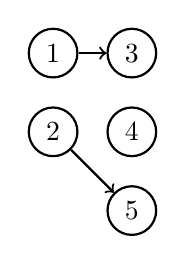
\begin{tikzpicture}[auto,
  specification/.style ={circle, draw, thick}]
 \node[specification] (A)  at (0,1)  {$1$};
 \node[specification] (B) at (0,0)  {$2$};
 \node[specification] (C)  at (1,1)  {$3$};
 \node[specification] (D)  at (1,0)  {$4$};
 \node[specification] (E)  at (1,-1)  {$5$};
 
 \draw[thick, ->] (A) to (C);
 \draw[thick, ->] (B) to (E);
\end{tikzpicture}
}

设$X$为有穷集合,$R$为集合$X$上的二元关系。当用图表示$R$时,先把$X$的元素在纸
上用点表示,并在其旁边标上这个元素的名字。然后把$R$的任一序对$(x,y)$用
从代表$x$的点画一条指向代表$y$的点的矢线表示。这样就得到了一个由点、线
组成的“有向图”,称为关系$R$的图。注意,如果$(x,x)\in R$,则在代表$x$的点画一条又指向此点的矢线,称为环。

设集合$X=\{1,2,3,4,5,6 \}$上的关系$R$定义如下:
    \begin{align*}
      R=&\{(1,1),(1,3),(1,5),(2,2),(2,4),(3,1),(3,3),(3,5),(4,2),\\
      &(4,4),(5,1),(5,3),(5,5),(6,6)\},
    \end{align*}
    则关系$R$的图为

{\centering
    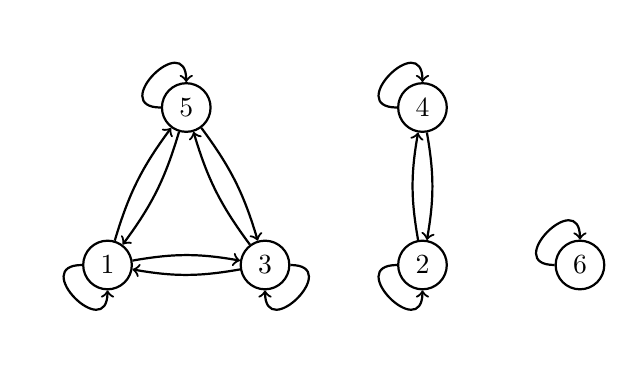
\begin{tikzpicture}[auto,
      specification/.style ={circle, draw, thick}]
     \node[specification] (A)  at (0,0)  {$1$};
     \node[specification] (B) at (2,0)  {$3$};
     \node[specification] (C)  at (1,2)  {$5$};
     \node[specification] (D)  at (4,0)  {$2$};
     \node[specification] (E)  at (4,2)  {$4$};
     \node[specification] (F)  at (6,0)  {$6$};
     
     \draw[thick, ->] (A) to [bend left = 10]  (B);
     \draw[thick, ->] (B) to [bend left = 10]  (A);
  
     \draw[thick, ->] (C) to [bend left = 10]  (B);
     \draw[thick, ->] (B) to [bend left = 10]  (C);
     
     
     \draw[thick, ->] (A) to [bend left = 10] (C);
     \draw[thick, ->] (C) to [bend left = 10] (A);
     
     \draw[thick, ->] (A) .. controls +(left:10mm) and +(down:10mm) ..  (A);
     \draw[thick, ->] (B) .. controls +(right:10mm) and +(down:10mm) ..  (B);
     \draw[thick, ->] (C) .. controls +(left:10mm) and  +(up:10mm) ..  (C);
  
     \draw[thick, ->] (D) to [bend left = 10] (E);
     \draw[thick, ->] (E) to [bend left = 10] (D);
     \draw[thick, ->] (D) .. controls +(left:10mm) and +(down:10mm) ..  (D);
     \draw[thick, ->] (E) .. controls +(left:10mm) and +(up:10mm) ..  (E);
     \draw[thick, ->] (F) .. controls +(left:10mm) and +(up:10mm) ..  (F);
  
  \end{tikzpicture}
}  

  \begin{Thm}
  设$R$为集合$X$上的二元关系,则
  \begin{enumerate}
  \item $R$为自反的,当且仅当$R$的图的每个顶点均有一个环;
  \item $R$为反自反的,当且仅当$R$的图中没有环;
  \item $R$为对称的,当且仅当$R$的图中任意两个不同顶点间有矢线,则必有两条方向相反的矢线;
  \item $R$为反对称的,当且仅当$R$的图中任意两个不同顶点间有矢线,则不能有两条方向相反的矢线;
  \item $R$为传递的,当且仅当在$R$的图中如果从某顶点沿矢线经两条矢线可到另一顶点,则从该顶点到另一顶点有一条矢线。
  \end{enumerate}
\end{Thm}

  \begin{Def}
    设$R$为集合$X$上的一个二元关系。$X$上的一切包含$R$的传递关系的交称为$R$的传递闭包,用$R^+$表示。即
    \begin{equation*}
      R^+ = \bigcap_{R \subseteq R' \text{且} R'\text{是传递的}}R'
    \end{equation*}
  \end{Def}
  \begin{Thm}
    设$R$为集合X上的一个二元关系,则关系$R$的传递闭包$R^+$为包含$R$的传递关系。
  \end{Thm}
\begin{proof}[证明]
    由定义$R^+ = \bigcap_{R \subseteq R' \text{且} R'\text{是传递的}}R'$,显然$R\subseteq R^+$。对任意的$x\in X$,$y\in X$,$z\in X$,$(x,y)\in R^+$并且$(y,z)\in R^+$,则对任意的$R'$,$R\subseteq R'$且$R'$是传递的
,$(x,y)\in R'$并且$(y,z)\in R'$,由$R'$为传递的知$(x,z)\in R'$,从而$(x,z)\in R^+$,这证明了$R^+$为传递的。
  \end{proof}



    \begin{Thm}
    设$R$为集合$X$上的一个二元关系,$a \in X$,$b \in X$,$n \geq 2$,则$(a,b) \in R^n$当且仅当存在$x_1\in X$,$x_2\in X$,$\ldots$,$x_{n-1}\in X$,使得$(a, x_1) \in R$,$(x_1, x_2)\in R$,  $\ldots$, $(x_{n-1}, b)\in R$。
  \end{Thm}
  \begin{proof}[证明]
  用数学归纳法证明,施归纳于$n$:

  当$n=2$时,由关系合成运算的定义知$(a,b)\in R^2$当且仅当存在$x_1\in X$使得$(a,x_1)\in R$且$(x_1, b)\in R$,结论成立。

   假设当$n=k$时定理的结论成立,往证当$n=k+1$时定理的结论也成立。
   由关系合成运算的定义知$(a,b)\in R^{k+1}$当且仅当存在$x\in X$使得$(a,x)\in R^k$且$(x, b)\in R$。 由归纳假设,$(a,x)\in R^k$当且仅当存在$x_1\in X$,$x_2\in X$,$\ldots$,$x_{k-1}\in X$,使得$(a, x_1) \in R$,$(x_1, x_2)\in R$,  $\ldots$, $(x_{k-1}, x)\in R$。 记$x_{k}=x$,则$(a,b)\in R^{k+1}$当且仅当存在$x_1\in X$,$x_2\in X$,$\ldots$,$x_{k-1}\in X$,$x_{k}\in X$,使得$(a, x_1) \in R,(x_1, x_2)\in R,\ldots,(x_{k-1}, x_k)\in R,(x_k, b)\in R$。
\end{proof}
  \begin{Thm}
    设$R$为集合$X$上的一个二元关系,则
    \begin{equation*}
      R^+ = \bigcup_{n=1}^\infty R^n = R \cup R^2 \cup R^3 \cup \cdots 
    \end{equation*}
  \end{Thm}
  \begin{proof}[证明]
    首先证明$ R^+ \subseteq \bigcup_{n=1}^\infty R^n$。

    由$R^+$的定义,只需证$\bigcup_{n=1}^\infty R^n$为包含$R$的传递关系即可。
    $R\subseteq \bigcup_{n=1}^\infty R^n$是显然的。以下证明$\bigcup_{n=1}^\infty R^n$为传递的。
    对任意的$a\in X$,$b\in X$,$c\in X$,如果$(a,b)\in \bigcup_{n=1}^\infty R^n$并且$(b,c)\in \bigcup_{n=1}^\infty R^n$,则存在正整数
    $m$和$n$使得$(a,b)\in R^m$且$(b,c)\in R^n$。于是$(a,c)\in R^m\circ R^n = R^{m+n}$,从而$(a,c)\in \bigcup_{n=1}^\infty R^n$。所以,
    $\bigcup_{n=1}^\infty R^n$是传递的。

    其次证明$  \bigcup_{n=1}^\infty R^n\subseteq R^+$。对任意的$a\in X$,$b\in X$,如果$(a,b)\in \bigcup_{n=1}^\infty R^n$,则存在某个正整数$m$,使得$(a,b)\in R^m$。
    如果$m=1$,则$(a,b)\in R\subseteq R^+$;如果$m>1$,则存在$b_1,b_2,\cdots, b_{m-1}\in X$使得
    $(a,b_1)\in R$,$(b_1,b_2)\in R$,$\ldots$,$(b_{m-1},b)\in R$。由$R\subseteq R^+$知$(a,b_1)\in R^+$,$(b_1,b_2)\in R^+$,$\ldots$,$(b_{m-1},b)\in R^+$。又因为$R^+$为传递的,所以$(a,b)\in R^+$。于是,$ \bigcup_{n=1}^\infty R^n\subseteq R^+$。

    因此,$ R^+ = \bigcup_{n=1}^\infty R^n$。
  \end{proof}
  \begin{Thm}
    设$R$为集合$X$上的一个二元关系,$|X| = n$,则\[R^+ = \bigcup_{i=1}^nR^i = R \cup R^2  \cup \cdots \cup R^n \]。
  \end{Thm}
  \begin{proof}[证明]
      只须证明对任一自然数$k > n$,有$R^k \subseteq \bigcup_{i=1}^nR^i$。
      为此,设$(a,b) \in R^k$,则存在$b_1, b_2, \cdots, b_{k-1} \in
      X$使得$(a,b_1) \in R$, $(b_1, b_2) \in R, \cdots, (b_{k-2}, b_{k-1})\in R,
      (b_{k-1}, b) \in R$。记$b_0 = a, b_k = b$。  $b_1,b_2, \cdots,
      b_{k-1}, b$是$X$中的$k$个元素,而$X$中仅有$n$个元素,$n < k$,所以$b_1,
      b_2, \cdots, b_{k-1}, b$中必有两个相等的元素。设$b_i=b_j$,$1 \leq i < j
      \leq k$。  于是,我们有$(a,b_1)\in R, \cdots, (b_{i-1}, b_i)\in R,
      (b_j, b_{j+1})\in R, \cdots, (b_{k-1},b)\in R$,故$(a,b)\in
      R^{k-(j-i)}$,$p_1=k-(j-i) < k$。  若$p_1 = k - (j - i) > n$, 则重复
      上述过程又有$p_2 < p_1$使得$(a,b) \in R^{p_2}$。  如此进行下去,必
      有$m \leq n$使得$(a,b) \in R^m$。所以,$R^k \subseteq
      \bigcup_{i=1}^nR^i$。  因此,$R^+=\bigcup_{i=1}^nR^i$。
  \end{proof}

    \begin{Thm}
    设$R$为集合$X$上的一个二元关系,$|X| = n$, $B$为$R$的关系矩阵,$B_{R^+}$为$R^+$的关系矩阵,简记为$B^+$,则
    \begin{equation*}
      B^+ = B \lor B^{(2)} \lor \cdots \lor B^{(n)}
    \end{equation*}
  \end{Thm}

  以下为计算集合$X$上关系$R$的传递闭包的算法。
   \begin{codebox}
    \Procname{$\proc{Transitive-Closure}(B)$}
    \zi \Comment $B$ is the zero-one $n \times n$ matrix for relation $R$
    \li $M \gets B$
    \li $A \gets M$
    \li \For $i \gets 2$ \To $n$
    \li \Do
        $M \gets M \circ B$
    \li $A \gets A \lor M$
    \End
    \li \Return A \Comment $A$ is the zero-one matrix for $R^+$
  \end{codebox}
  \begin{codebox}
    \Procname{$\proc{Warshall}(B)$}
    \zi \Comment $B$ is the zero-one $n \times n$ matrix for relation $R$
    \li $A \gets B$
    \li \For $k \gets 1$ \To $n$
    \li \Do
    \For $i \gets 1$ \To $n$
    \li \Do
    \For $j \gets 1$ \To $n$
    \li \Do
    $a_{ij} = a_{ij} \lor (a_{ik} \land a_{kj})$
    \End
    \End
    \End
    \li \Return A \Comment $A$ is the zero-one matrix for $R^+$
  \end{codebox}  

  $X=\{x_1,x_2,\cdots,x_n\}$

  $a_{ij}^{(0)}=a_{ij}$


  $a_{ij}^{(k)}= a_{ij}^{(k-1)}\lor (a_{ik}^{(k-1)}\land a_{kj}^{(k-1)}) (k\geq 1)$

  其中$a_{ij}^{(k)}=1$当且仅当存在$x_{i_1},x_{i_2},\ldots,x_{i_m}\in \{x_1,x_2,\ldots,x_k\}$使得$(x_i,x_{i_1})\in R$,$(x_{i_1},x_{i_2})\in R$,$\cdots$,$(x_{i_m},x_j)\in R$。


  $a_{ik} = a_{ik} \lor (a_{ik} \land a_{kk})$

  $a_{kj} = a_{kj} \lor (a_{kk} \land a_{kj})$

    \begin{codebox}
    \Procname{$\proc{Warshall}(B)$}
    \zi \Comment $B$ is the zero-one $n \times n$ matrix for relation $R$
    \li $A \gets B$
    \li \For $k \gets 1$ \To $n$
    \li \Do
    \For $i \gets 1$ \To $n$
    \li \Do
     \If $a_{ik} \isequal 1$
    \li \Then
    \For $j \gets 1$ \To $n$
    \li \Do
    $a_{ij} = a_{ij} \lor a_{kj}$
    \End
    \End
    \End
    \End
    \li \Return A \Comment $A$ is the zero-one matrix for $R^+$
  \end{codebox}
  \begin{Def}
    集合$X$上的二元关系$R$称为{\bfseries 等价关系},如果$R$同时满足以下三个性质:
    \begin{enumerate}
    \item $R$为自反的,即对$X$中的任意元素$x$,$xRx$;
    \item $R$为对称的,即对$X$中的任意元素$x$,$y$,如果$xRy$,则$yRx$;
    \item $R$为传递的,即对$X$中的任意元素$x$,$y$,$z$,如果$xRy$且$yRz$,则$xRz$。
    \end{enumerate}
  \end{Def}

  这是在我们这门课中迄今为止所学的所有概念中最重要的概念之一,是不是有点抽象?我们可以借助一个具体的例子,帮助我们理解这些抽象的概念。从小学到现在,我们是不是学了许多类似于“$\frac{1}{4}+\frac{1}{4}=\frac{1}{2}$”的等式?这里的等价关系就是从“$=$”抽象出来的。(1)$x=x$;(2)如果$x=y$,那么$y=x$;(3)如果$x=y$并且$y=z$,那么$x=z$。是不是显然成立呀?我们可以借助熟知的"="来理解等价关系的定义。
  \begin{Def}
    设$a,b\in Z$,如果存在$q\in Z$使得$a=qb$,则称$b$整除$a$,记为$b|a$。
  \end{Def}
  \begin{Def}
    设$a,b\in Z$,$b>0$,$a=qb+r$,$q\in Z$,$0\leq r<b$,则称$r$为$a$除以$b$所得到的余数,记为$a\bmod b$。
  \end{Def}
  
  \begin{Def}
    设$a,b,n\in Z$,$n>0$,如果$a\bmod n=b\bmod n$,则称$a$与$b$模$n$同余,记为$a \equiv b\pmod{n}$。
  \end{Def}
  
  \begin{Thm}
    $\forall a,b,n\in Z, n>0, a\equiv b\pmod{n}$等价于$n|(a-b)$。
  \end{Thm}
  
  \begin{Example}\label{mod}
    整数集$\mathbb{Z}$上的模$n$同余关系为$\mathbb{Z}$上的等价关系。
  \end{Example}
  
  
  \begin{Example}\label{number}
    设集合
    $X=\{1,2,3,4,5,6 \}$上的关系$R$定义如下:
    \begin{align*}
      R=&\{(1,1),(1,3),(1,5),(2,2),(2,4),(3,1),(3,3),(3,5),(4,2),\\
      &(4,4),(5,1),(5,3),(5,5),(6,6)\},
    \end{align*}
      则$R$为$X$上的等价关系。
    \end{Example}
    \begin{proof}[证法一]
      直接根据定义进行验证。
    \end{proof}
    \begin{proof}[证法二]
      画出$R$的关系图进行判断。

      
        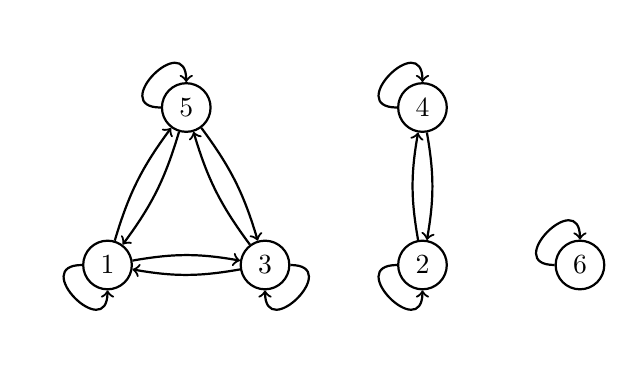
\begin{tikzpicture}[auto,
    specification/.style ={circle, draw, thick}]
   \node[specification] (A)  at (0,0)  {$1$};
   \node[specification] (B) at (2,0)  {$3$};
   \node[specification] (C)  at (1,2)  {$5$};
   \node[specification] (D)  at (4,0)  {$2$};
   \node[specification] (E)  at (4,2)  {$4$};
   \node[specification] (F)  at (6,0)  {$6$};
   
   \draw[thick, ->] (A) to [bend left = 10]  (B);
   \draw[thick, ->] (B) to [bend left = 10]  (A);

   \draw[thick, ->] (C) to [bend left = 10]  (B);
   \draw[thick, ->] (B) to [bend left = 10]  (C);
   
   
   \draw[thick, ->] (A) to [bend left = 10] (C);
   \draw[thick, ->] (C) to [bend left = 10] (A);
   
   \draw[thick, ->] (A) .. controls +(left:10mm) and +(down:10mm) ..  (A);
   \draw[thick, ->] (B) .. controls +(right:10mm) and +(down:10mm) ..  (B);
   \draw[thick, ->] (C) .. controls +(left:10mm) and  +(up:10mm) ..  (C);

   \draw[thick, ->] (D) to [bend left = 10] (E);
   \draw[thick, ->] (E) to [bend left = 10] (D);
   \draw[thick, ->] (D) .. controls +(left:10mm) and +(down:10mm) ..  (D);
   \draw[thick, ->] (E) .. controls +(left:10mm) and +(up:10mm) ..  (E);
   \draw[thick, ->] (F) .. controls +(left:10mm) and +(up:10mm) ..  (F);

\end{tikzpicture}

  
  (1)在$R$的图中,每个顶点均有一个环,这说明$R$为自反的;
  
  (2)在$R$的图中,如果任意两个不同顶点间有矢线,则必有两条方向相反的矢线,这说明$R$为对称的;

  (3)在$R$的图中,如果从某顶点沿矢线经两条矢线可到另一顶点,则从该顶点到另一顶点有一条矢线,这说明$R$为传递的。

    \end{proof}
    如果我们写个程序进行判断,首先要将该二元关系在计算机中表示出来。矩阵表示法为我们提供了一种解决方案。
    \begin{proof}[证法三]
      关系$R$的矩阵表示为
      \[B=\begin{bmatrix}
          1&0&1&0&1&0\\
          0&1&0&1&0&0\\
          1&0&1&0&1&0\\
          0&1&0&1&0&0\\
          1&0&1&0&1&0\\
          0&0&0&0&0&1
        \end{bmatrix}
      \]

      (1)$B$的对角线上的元素全为$1$说明$R$为自反的;

      (2)$B$为对称矩阵说明$R$为对称的;

      (3)

      \[B\circ B=\begin{bmatrix}
          1&0&1&0&1&0\\
          0&1&0&1&0&0\\
          1&0&1&0&1&0\\
          0&1&0&1&0&0\\
          1&0&1&0&1&0\\
          0&0&0&0&0&1
        \end{bmatrix}\circ\begin{bmatrix}
          1&0&1&0&1&0\\
          0&1&0&1&0&0\\
          1&0&1&0&1&0\\
          0&1&0&1&0&0\\
          1&0&1&0&1&0\\
          0&0&0&0&0&1
        \end{bmatrix}=\begin{bmatrix}
          1&0&1&0&1&0\\
          0&1&0&1&0&0\\
          1&0&1&0&1&0\\
          0&1&0&1&0&0\\
          1&0&1&0&1&0\\
          0&0&0&0&0&1
        \end{bmatrix}
      \]
      由$B\circ B$中的每个元素小于等于$B$中的每个元素知$R$为传递的。
    \end{proof}
  \begin{Def}
    设$\cong$为集合$X$上的一个等价关系,$x\in X$,$X$的子集
    \[E_x=\{y\in X | x \cong y\}\]称为$x$关于$\cong$的等价类,记为$[x]$,即
    \begin{equation*}
      [x] = \{y \in X | x \cong y\}
    \end{equation*}
  \end{Def}
  \begin{Example}
    在例\ref{mod}中我们已经知道模$4$同余关系为等价关系,试写出其所有等价类所构成的集合。
  \end{Example}
  \begin{proof}[解]
    模$4$同余关系所有等价类所构成的集合为$\{[0],[1],[2],[3]\}$,其中
    \begin{align*}
      [0]&=\{\cdots,-8,-4,0,4,8,\cdots\}\\
      [1]&=\{\cdots,-7,-3,1,5,9,\cdots\}\\
      [2]&=\{\cdots,-6,-2,2,6,10,\cdots\}\\
      [3]&=\{\cdots,-5,-1,3,7,11,\cdots\}
    \end{align*}
  \end{proof}
  \begin{Example}
    设集合
    $X=\{1,2,3,4,5,6 \}$上的关系$R$定义如下:
    \begin{align*}
      R=&\{(1,1),(1,3),(1,5),(2,2),(2,4),(3,1),(3,3),(3,5),(4,2),\\
      &(4,4),(5,1),(5,3),(5,5),(6,6)\},
    \end{align*}
      在例\ref{number}中,我们知道$R$为$X$上的等价关系,试写出其所有等价类所构成的集合。
    \end{Example}
    \begin{proof}[解]
      我们先尝试写出集合$X$上每个元素关于关系$R$的等价类:
      \begin{align*}
        [1]&=\{1,3,5\}\\
        [2]&=\{2,4\}\\
        [3]&=\{1,3,5\}\\
        [4]&=\{2,4\}\\
        [5]&=\{1,3,5\}\\
        [6]&=\{6\}
      \end{align*}
      你发现了什么?有重复!于是关系$R$的所有等价类所构成的集合为$\{[1],[2],[6]\}$, 即$\{\{1,3,5\},\{2,4\},\{6\}\}$。
    \end{proof}
    通过以上的例子,我们发现了以下的结论:
    \begin{Thm}
      设$\cong$为集合$X$上的一个等价关系,对任意的$x\in X$,$y\in X$,$x\cong y$当且仅当$[x]=[y]$。
    \end{Thm}
    \begin{proof}[证明]

      对任意的$x\in X$,$y\in X$,由$x\cong y$往证$[x]=[y]$。这里是要证明两个集合相等。对任意的$z\in [x]$,则$x\cong z$,由$x\cong y$及$\cong$的对称性知$y\cong x$,再由$\cong$的传递性知$y\cong z$,从而$z\in [y]$。对任意的$z\in [y]$,则$y\cong z$,由$x\cong y$及$\cong$的传递性知$x\cong z$,从而$z\in [x]$。这证明了$[x]=[y]$。

      对任意的$x\in X$,$y\in X$,由$[x]=[y]$往证$x\cong y$。由$\cong$的自反性知$x\cong x$,从而$x\in [x]$,再由$[x]=[y]$知$x\in [y]$,从而$y\cong x$,由$\cong$的对称性得$x\cong y$。
    \end{proof}
   \begin{Def}
    设$X$为集合, $X$的一些非空子集形成的集族$\mathscr{A}$称为$X$的一个{\bfseries 划分},如果$\mathscr{A}$具有性质
    \begin{enumerate}
    \item $\forall A, B \in \mathscr{A}$,如果$A \neq B$,则$A \cap B = \phi$;
      \item $\bigcup_{A \in \mathscr{A}} A= X$
    \end{enumerate}
  \end{Def}

  \begin{Example}
    集合
    \begin{equation*}
      \begin{split}
      \{&\{\cdots,-8,-4,0,4,8,\cdots\},\\
      &\{\cdots,-7,-3,1,5,9,\cdots\},\\
      &\{\cdots,-6,-2,2,6,10,\cdots\},\\
      &\{\cdots,-5,-1,3,7,11,\cdots\}\}
    \end{split}
  \end{equation*}
构成了整数集$\mathbb{Z}$的一个划分。
\end{Example}

  \begin{Example}
    集合$\{\{1,3,5\},\{2,4\},\{6\}\}$
构成了集合$X=\{1,2,3,4,5,6\}$的一个划分。
  \end{Example}

  \begin{Thm}\label{thm1}
    设$\cong$为集合$X$上的一个等价关系,则$\cong$的所有等价类的集合构成了集合$X$的一个划分。
  \end{Thm}
  \begin{proof}[证明]
    这就是要证明$\{[x]|x\in X\}$构成了集合$X$的一个划分。

    对任意的$x\in X$,由$\cong$的自反性知$x\cong x$,从而$x\in [x]$,这证明了$[x]$非空。

    对任意的$x\in X$,$y\in X$,如果$[x]\neq [y]$,以下证明$[x]\cap [y]=\phi$。用反证法,假设$[x]\cap [y]\neq \phi$,则存在$z\in [x]\cap [y]$,于是$z\in [x]$并且$z\in [y]$。由$z\in [x]$知$x\cong z$,由$z\in [y]$知$y\cong z$。由$\cong$的对称性可得$z\cong y$,再由$\cong$的传递性可得$x\cong y$,从而$[x]=[y]$,矛盾。

    由对任意的$x\in X$,$x\in [x]$易知$\bigcup_{x\in X}[x]=X$。

    综上,我们证明了$\{[x]|x\in X\}$构成了集合$X$的一个划分。
  \end{proof}
  \begin{Thm}\label{thm2}
    设$\mathscr{A}$为集合$X$的一个划分,令\[\cong = \bigcup_{A\in \mathscr{A}}A\times A\]
    则$\cong$为集合$X$上的一个等价关系。
  \end{Thm}
  这个定理的符号不太好理解吧?在以后学习的过程中,遇到类似这个定理中的抽象的符号应该怎么办?具体的例子可以帮助我们很好的理解这些抽象的符号。例如,设集合$X=\{1,2,3,4,5,6\}$, $\mathscr{A}=\{\{1,3,5\},\{2,4\},\{6\}\}$为集合$X$的一个划分,则
  \begin{equation*}
    \begin{split}
      &\bigcup_{A\in \mathscr{A}}A\times A\\
      =&(\{1,3,5\} \times \{1,3,5\}) \cup (\{2,4\}\times \{2,4\}) \cup (\{6\}\times \{6\})\\
      =&\{(1,1),(1,3),(1,5),(3,1),(3,3),(3,5),(5,1),(5,3),(5,5),(2,2),(2,4),(4,2),(4,4),(6,6)\}
    \end{split}
  \end{equation*}
  为集合$X$上的一个等价关系。

  \begin{proof}[证明]
    这就是要验证$\cong$满足自反性、对称性和传递性。

    (1)对任意的$x\in X$,由$\mathscr{A}$为集合$X$的一个划分知存在$A\in \mathscr{A}$使得$x\in A$,从而$(x,x) \in A\times A$,于是, $(x,x)\in \bigcup_{A\in \mathscr{A}}A\times A$,这说明$\cong$满足自反性。

    (2)对任意的$x\in X$,$y\in X$,如果$(x,y)\in \bigcup_{A\in \mathscr{A}}A\times A$,那么存在$A\in \mathscr{A}$使得$(x,y)\in A\times A$,从而$(y,x)\in A\times A$,于是$(y,x)\in \bigcup_{A\in \mathscr{A}}A\times A$,这说明$\cong$满足对称性。

    (3)对任意的$x\in X$,$y\in X$,$z\in X$,如果$(x,y)\in \bigcup_{A\in \mathscr{A}}A\times A$,并且$(y,z)\in \bigcup_{A\in \mathscr{A}}A\times A$,那么存在$A\in \mathscr{A}$使得$(x,y)\in A\times A$,并且存在$B\in \mathscr{A}$使得$(y,z)\in B\times B$。于是,$x\in A$,$y\in A$,$y\in B$,$z\in B$。此时,必有$A=B$,否则$A\cap B=\phi$,这与$y\in A$并且$y\in B$矛盾。从而,$x\in A$,$z\in A$,因此,$(x,z)\in A\times A$,于是$(x,z)\in \bigcup_{A\in \mathscr{A}}A\times A$,这说明$\cong$满足传递性。
    
  \end{proof}

  本门课一个很重要的结论为“集合$X$上的所有等价关系之集与集合$X$的所有划分之集之间存在着一一对应的关系”。为了证明这个结论,我们需要构造一个从集合$X$上的所有等价关系之集到集合$X$的所有划分之集之间的一个双射。还记得我们学过的可逆映射的概念吗?一个映射为双射,当且仅当为该映射为可逆映射。于是我们可以构造一个从集合$X$上的所有等价关系之集到集合$X$的所有划分之集之间的一个可逆映射。还记得可逆映射的定义吗?

       设$f:X\to Y$为一个映射。如果存在一个映射$g:Y\to X$使得\[f\circ g = I_{Y} \text{且} g\circ f = I_{X},\]则称映射$f$为可逆的,而$g$称为$f$的逆映射。
借助于以上我们所学过的数学概念,我们有如下的定理:
 \begin{Thm}
    设$X$为一个集合,
    \begin{align*}
    \mathbb{R} &= \{\cong \subseteq X \times X | \cong\text{为集合}X\text{上的一个等价关系}\},\\
      \mathbb{A} &= \{\mathscr{A} \subseteq 2^X| \mathscr{A}\text{为集合}X\text{的一个划分}\},\\
      f &= \{(\cong, \{[x]_{\cong} | x \in X\})|\cong \in \mathbb{R}, [x]_{\cong}=\{y\in X | x \cong y\}\}\\
      g&=\{(\mathscr{A}, \bigcup_{A \in \mathscr{A}}A\times A)|\mathscr{A} \in \mathbb{A}\}
    \end{align*}
    则$f$为从$\mathbb{R}$到$\mathbb{A}$的双射,且$f^{-1}=g$。
  \end{Thm}
  如果我们能够完全理解该定理,并能够从“0”开始给出该定理的证明过程,即该定理所依赖的其他结论都可以给出证明,那么,整个前三章的内容,我们就有了一个很好的把握了。集中精力搞懂本课程的一些重要定理的证明过程,顺藤摸瓜,这些定理所依赖的其他结论也能够给出证明,直到可以从头开始说起,这对于提升我们的逻辑思维能力是很有帮助的。

  这是我们所遇到的第一个重要的定理。让我们先从理解这个定理开始吧。还记得我们应该怎样理解抽象的符号和术语吗?答案是尝试具体的例子。

  让我们尝试一个简单的集合:$X=\{1,2,3\}$。那么$\mathbb{R}$表示集合$X$上所有的等价关系构成的集合,这个集合是怎样的?这个问题不好回答吧?

  让我们先看$\mathbb{A}$吧。$\mathbb{A}$表示集合$X$的所有划分构成的集合。这个集合比较好写,你能写出答案吗?我的答案是这样的:

  \begin{equation*}
    \begin{split}
      \mathbb{A}=\{&\{\{1\},\{2\},\{3\}\},\\
      &\{\{1,2\},\{3\}\},\\
      &\{\{1,3\},\{2\}\},\\
      &\{\{2,3\},\{1\}\},\\
      &\{\{1,2,3\}\}\}
    \end{split}
  \end{equation*}

  对任意的$\mathscr{A}\in \mathbb{A}$,我们计算$\bigcup_{A \in \mathscr{A}}A\times A$,就可以得到$X$上的一个等价关系。该定理是在说,在$\mathbb{R}$和$\mathbb{A}$之间存在一个一一对应的关系,于是,我们有
  \begin{equation*}
    \begin{split}
      \mathbb{R}=\{&\{(1,1),(2,2),(3,3)\},\\
      &\{(1,1),(1,2),(2,1),(2,2),(3,3)\},\\
      &\{(1,1),(1,3),(3,1),(3,3),(2,2)\},\\
      &\{(2,2),(2,3),(3,2),(3,3),(1,1)\},\\
      &\{(1,1),(1,2),(1,3),(2,1),(2,2),(2,3),(3,1),(3,2),(3,3)\}\}      
    \end{split}
  \end{equation*}
  \begin{proof}[证明]
    \begin{enumerate}
    \item 证明$f$为映射。这就是要证明对于集合$X$上的任意一个等价关系$\cong$, 
      $\{[x]_{\cong}|x\in X\}$为集合$X$的一个划分。这就是定理\ref{thm1}。
    \item 证明$g$为映射。这就是要证明对于集合$X$的任意一个划分$\mathscr{A}$,
      $\bigcup_{A\in \mathscr{A}}A\times A$为集合$X$上的一个等价关系。这就是定理\ref{thm2}。
    \item 证明$g\circ f = I_{\mathbb{R}}$。这就是要证明对于集合$X$上的任意一个等
      价关系$\cong$,$\bigcup_{x\in X}[x]_{\cong}\times [x]_{\cong} = \cong$。

      这里是要证明两个集合相等。

      对任意的$x_1\in X$,$x_2\in X$,如果$(x_1,x_2)\in \bigcup_{x\in X}[x]_{\cong}\times [x]_{\cong}$,那么存在$x\in X$,$(x_1,x_2)\in [x]_{\cong}\times [x]_{\cong}$,于是$x_1\in [x]_{\cong}$并且$x_2\in [x]_{\cong}$,从而$x\cong x_1$并且$x\cong x_2$,由$\cong$的对称性知$x_1\cong x$,再由$\cong$的传递性知$x_1\cong x_2$,即$(x_1,x_2)\in \cong$。

      对任意的$x_1\in X$,$x_2\in X$,如果$(x_1,x_2)\in \cong$,则$x_1\cong x_2$,从而$x_2\in [x_1]_{\cong}$,由$\cong$的自反性知$x_1\cong x_1$,从而$x_1\in [x_1]_{\cong}$。于是,$(x_1,x_2)\in [x_1]_{\cong}\times [x_1]_{\cong}\subseteq \bigcup_{x\in X}[x]_{\cong}\times [x]_{\cong}$。
    \item 证明$f\circ g = I_{\mathbb{A}}$。这就是要证明对于集合$X$上的任意一个划分
      $\mathscr{A}$,关于等价关系$\bigcup_{A \in \mathscr{A}}A\times A$的等价类
      的集合就是$\mathscr{A}$。

      这里还是要证明两个集合相等。

      对任意的$x\in X$,设$[x]$为关于等价关系$\bigcup_{A \in \mathscr{A}}A\times A$的一个等价类,以下证明$[x]\in \mathscr{A}$。由$\bigcup_{A\in \mathscr{A}}A=X$知存在$A\in \mathscr{A}$使得$x\in A$。如果我们能够证明$[x]=A$,则$[x]\in \mathscr{A}$得证。对任意的$y\in [x]$,则$(x,y)\in \bigcup_{A \in \mathscr{A}}A\times A$。于是,存在$B\in \mathscr{A}$使得$(x,y)\in B\times B$,如果$B\neq A$,那么$x\in A$且$x\in B$,这与$A\cap B=\phi$矛盾,从而$B=A$,因此$y\in A$。反之,对任意的$y\in A$,则$(x,y)\in \bigcup_{A \in \mathscr{A}}A\times A$,从而$y\in [x]$。这证明了$[x]=A$,从而$[x]\in \mathscr{A}$。

      对任意的$A\in \mathscr{A}$,以下证明$A$为等价关系$\bigcup_{A \in \mathscr{A}}A\times A$的一个等价类。由$A$非空知,存在$x$,$x\in A$,以下证明$A=[x]$,这里$[x]$表示$x$关于等价关系$\bigcup_{A \in \mathscr{A}}A\times A$的一个等价类。对任意的$y\in A$,则$(x,y)\in A\times A \subseteq \bigcup_{A \in \mathscr{A}}A\times A$,从而$y\in [x]$。反之,如果$y\in [x]$,则由与前面相类似的,可以证明$y\in A$。这证明了$A=[x]$。
    \end{enumerate}
  \end{proof}
  \begin{Def}
    设$\cong$为$X$上的等价关系,$\cong$的所有等价类之集称为$X$对$\cong$的商集,记为$X/\cong$。即
    \[X/\cong = \{[x]|x\in X,[x]\text{为}x\text{关于}\cong \text{的等价类}\}\]
  \end{Def}

  \begin{Example}
    设集合$X=\{1,2,3,4,5,6\}$,$\cong$为集合$X$的等价关系,$X/\cong=\{\{1,2\},\{3,5\},\{4,6\}\}$,试求$\cong$。
  \end{Example}

  \begin{Exercise}
    设$X = \{1,2,3\}$, $Y = \{1,2\}$,$S = \{f|f:X \to Y\}$。$S$上的二元关系$\cong$定义如下:$\forall f,g\in S$,$f \cong g$当且仅当\[I_m(f) = I_m(g)\]证明$\cong$是$S$上的等价关系,并求出等价类之集。      
   \end{Exercise}
   \begin{proof}[解]
     首先验证$\cong$为$S$上的等价关系:
     
     $\cong$为自反的,这是因为对任意的映射$f:X\to Y$,$I_m(f)=I_m(f)$;
 
     $\cong$为对称的,这是因为对任意的映射$f:X\to Y$,$g:X\to Y$,如果$I_m(f)=I_m(g)$,则$I_m(g)=I_m(f)$;
 
     $\cong$为传递的,这是因为对任意的映射$f:X\to Y$,$g:X\to Y$,$h:X\to Y$,如果$I_m(f)=I_m(g)$并且$I_m(g)=I_m(h)$,则$I_m(f)=I_m(h)$。
     
     $S=\{f_1,f_2,f_3,f_4,f_5,f_6,f_7,f_8\}$,
     其中
     \begin{align*}
       &f_1:X\to Y, f_1(1)=1,f_1(2)=1,f_1(3) = 1, Im(f_1)=\{1\}\\
       &f_2:X\to Y, f_2(1)=1,f_2(2)=1,f_2(3) = 2, Im(f_2)=\{1,2\}\\
       &f_3:X\to Y, f_3(1)=1,f_3(2)=2,f_3(3) = 1, Im(f_3)=\{1,2\}\\
       &f_4:X\to Y, f_4(1)=1,f_4(2)=2,f_4(3) = 2, Im(f_4)=\{1,2\}\\
       &f_5:X\to Y, f_5(1)=2,f_5(2)=1,f_5(3) = 1, Im(f_5)=\{1,2\}\\
       &f_6:X\to Y, f_6(1)=2,f_6(2)=1,f_6(3) = 2, Im(f_6)=\{1,2\}\\
       &f_7:X\to Y, f_7(1)=2,f_7(2)=2,f_7(3) = 1, Im(f_7)=\{1,2\}\\
       &f_8:X\to Y, f_8(1)=2,f_8(2)=2,f_8(3) = 2, Im(f_8)=\{2\}\\
     \end{align*}
     则$S/\cong=\{\{f_1\},\{f_2,f_3,f_4,f_5,f_6,f_7\},\{f_8\}\}$
   \end{proof}
 
  \begin{Def}
    集合$X$上的二元关系$R$称为{\bfseries 偏序关系},如果$R$同时满足以下三个性质:
    \begin{enumerate}
    \item $R$为自反的,即对$X$中的任意元素$x$,$xRx$;
    \item $R$为反对称的,即对$X$中的任意元素$x$,$y$,如果$xRy$且$yRx$,则$x=y$;
    \item $R$为传递的,即对$X$中的任意元素$x$,$y$,$z$,如果$xRy$且$yRz$,则$xRz$。
    \end{enumerate}
  \end{Def}
    \begin{Def}
    设$\leq$为集合$X$上的一个偏序关系,则称二元组$(X,\leq)$为一个{\bfseries 偏序集}。
  \end{Def}

    \begin{Example}
    实数集$\mathbb{R}$上通常的“小于等于”关系$\leq$为一个偏序关系,所以$(\mathbb{R},\leq)$为一个偏序集。
  \end{Example}
  \begin{Example}
    设$S$为一个集合,$S$的子集间的包含关系$\subseteq$为$2^S$上的一个偏序关系,所以$(2^{\mathbb{S}},\subseteq)$为一个偏序集。
  \end{Example}

  \begin{Example}
    设集合
    $X=\{a,b,c,d\}$上的关系$R$定义如下:
    \begin{equation*}
      R=\{(a,a),(a,b),(a,c),(a,d),(b,b),(b,d),(c,c),(c,d),(d,d)\}
    \end{equation*}
  \end{Example}
  则$R$为$X$上的偏序关系。

  设$\leq$为集合$X$上的一个偏序关系。由于$\leq$为自反的,所以$\leq$的关系图中每个顶点
  都有一个环,略去每个顶点的环;由于$\leq$为传递的,如果$x\leq y$,且$y\leq z$,略去从顶点$x$到顶点$z$的矢线;由于$\leq$为反对称的,如果从顶点$x$到顶点$y$有矢线,则将顶点$y$画在顶点$x$的
  上方,并略去矢线的箭头。按这种方法画出的图称为$(X,\leq)$的哈斯图(Hasse图)。

  \begin{Example}
    设$X=\{1,2,3\}$,画出偏序集$(2^X,\subseteq)$的哈斯图。
  \end{Example}
  {\centering
  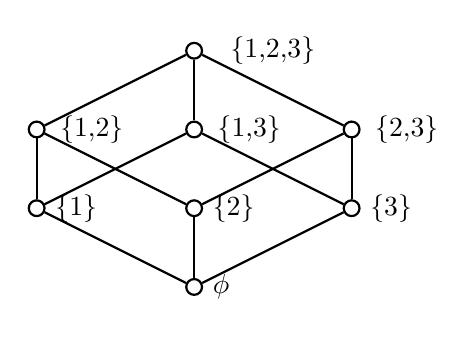
\begin{tikzpicture}[auto,
  specification/.style ={circle, draw, thick, inner sep = 0pt, minimum size=2mm}]
 \node[specification] (A)  [label=0:$\phi$] at (0,0)  {};
 \node[specification] (B)  [label=0:$\{1\}$] at (-2,1)  {};
 \node[specification] (C)  [label=0:$\{2\}$] at (0,1)  {};
 \node[specification] (D) [label=0:$\{3\}$] at (2,1)  {};
 \node[specification] (E)   at (-2,2)  {};
 \node at (-1.3,2) {\{1,2\}};  
 \node[specification] (F)   at (0,2)  {};
 \node at (0.7,2) {\{1,3\}};  
 \node[specification] (G)  at (2,2)  {};
 \node at (2.7,2) {\{2,3\}};  
 \node[specification] (H)   at (0,3)  {};
 \node at (1,3) {\{1,2,3\}};
 \draw[thick] (A) to  (B);
 \draw[thick] (A) to  (C);
 \draw[thick] (A) to  (D);
 \draw[thick] (B) to  (E);
 \draw[thick] (B) to  (F);
 \draw[thick] (C) to  (E);
 \draw[thick] (C) to  (G);
 \draw[thick] (D) to  (F);
 \draw[thick] (D) to  (G);
 \draw[thick] (E) to  (H);
 \draw[thick] (F) to  (H);
 \draw[thick] (G) to  (H);
\end{tikzpicture}
  }

    \begin{Def}
    设$\leq$为集合$X$上的偏序关系,如果$\forall x, y \in X$,$x \leq y$与$y \leq x$至少有一个成立,则称$\leq$为$X$上的全序关系。相应的,二元组$(X,\leq)$称为全序集。
  \end{Def}
  我们用$x<y$表示$x\leq y$并且$x\neq y$,$x\geq y$表示$y\leq x$,$x > y$表示$x\geq y$并且$x\neq y$。

  \begin{Def}
    设$(X,\leq)$为一个偏序集,$A\subseteq X$。如果存在一个元素$s\in A$使得$\forall x \in A$有$s\geq x$,则称$s$为$A$的{\bfseries 最大元素};如果存在一个元素$t\in A$使得$\forall x \in A$有$t \leq x$,则称$t$为$A$的{\bfseries 最小元素}。
  \end{Def}

  
    \begin{Def}
    设$(X,\leq)$为一个偏序集,$A\subseteq X$。如果存在一个元素$s\in A$,在$A$中没
    有元素$x$使得$x > s$,则称$s$为$A$的{\bfseries 极大元素};如果存在一个元素$t\in A$,在$A$中没有元素$x$使得$x < t$,则称$t$为$A$的{\bfseries 极小元素}。
  \end{Def}

    \begin{Def}
    设$(X,\leq)$为一个偏序集,$A\subseteq X$。如果存在一个元素$s\in X$使得$\forall x \in A$有$s\geq x$,则称$s$为$A$的一个{\bfseries 上界};如果存在一个元素$t\in X$使得$\forall x \in A$有$t \leq x$,则称$t$为$A$的一个{\bfseries 下界}。
  \end{Def}
    \begin{Def}
      设$(X,\leq)$为一个偏序集,$A\subseteq X$。如果$A$有上界且$A$的一切上界之集有最小元素,则这个最小上界称为$A$的{\bfseries 上确界},记为$\sup A$;如果$A$有下界且$A$的一切下界之集有最大元素,则这个最大下界称为$A$的{\bfseries 下确界},记为$\inf A$。
  \end{Def}
\begin{Def}
  设$(X,\leq)$为一个偏序集,$A\subseteq X$。如果$\forall a,b\in A$,$a\leq b$与$b\leq a$必有一个成立,则称$A$为$X$中的链;如果对$A$中任意两个不同的元素$a$和$b$,$a\leq b$与$b\leq a$均不成立,则称$A$为$X$中的一个反链。$|A|$称为链(反链)的长度。
\end{Def}
  \begin{Thm}
    设$(X,\leq)$为一个偏序集,如果$X$中所有链长度的最大值为$n$,则$X$的全部元素可以被分成$n$个非空不相交反链的并集。
  \end{Thm}
  \begin{proof}[证明]
    用数学归纳法证明,施归纳于$n$。

    当$n=1$时,$X$中最长链的长度为$1$,所以$X$中任意两个不同的元素不能比较,从而,
    $X$就是反链,故定理的结论成立。

    假设当$n=k(k\geq 1)$时结论成立,往证当$n=k+1$时结论也成立。设$(X,\leq)$中最长链的长度为$k+1$,
    则$X$中有极大元。令$M$为$X$的所有极大元之集,则$M\neq \phi$且$M\neq X$。易证$X\setminus M$中最长链的长度为$k$。
    由归纳假设,$X\setminus M$可分解成$k$个非空不相交反链之并。$M$也是一个非空反链,所以$X$可以被分解成$k+1$个非空不相交反链之并。
  \end{proof}
  \begin{Cor}
    设$(X,\leq)$为一个偏序集,$|X|=mn+1$,则$X$中或存在一个长至少为$n+1$的链,或存在一个长至少为$m+1$的反链。
  \end{Cor}
  \begin{proof}[证明]
       用反证法。假设结论不成立,则$X$中每个链的长度$\leq n$,并且每个反链的长度$\leq m$。
       设$X$中最长链的长度为$k$,则$X$能被分成$k$个不相交反链之并。这里$k\leq n$,再由每个反链的长度$\leq m$,
        可以得到\[|X|\leq km \leq mn\]
        这与假设$|X|=mn+1$矛盾。
  \end{proof}
  \begin{Example}
    证明:每个由$n^2+1$个实数组成的序列$a_1,a_2,\cdots,a_{n^2+1}$中必有长至少为$n+1$的不减子序列,或有一个长至少为$n+1$的不增子序列。
  \end{Example}
\begin{proof}[证明]
  记$A=\{(a_i,i)|1\leq i \leq n^2+1\}$,在$A$上定义二元关系$\leq'$为:$(a_i,i)\leq'(a_j,j)$当且仅当$a_i\leq a_j$并且$i\leq j$,
  这里$\leq$为实数间通常的小于等于关系。

  易验证$\leq'$为自反的,反对称的和传递的,从而为集合$A$上的偏序关系。

  $A$中或有长为$n+1$的链,或有长为$n+1$的反链。如果$A$中有长为$n+1$的链$\{(a_{i_1},i_1),(a_{i_2},i_2),\cdots, (a_{i_{n+1}},i_{n+1})\}$,这里$i_1<i_2<\ldots<i_{n+1}$,则$a_{i_1},a_{i_2},\cdots,a_{i_n}$为
  序列$a_1,a_2,\ldots,a_{n^2+1}$的不减子序列。如果$A$中有长为$n+1$的反链$\{(a_{j_1},j_1),(a_{j_2},j_2),\cdots, (a_{j_{n+1}},j_{n+1})\}$,这里$j_1<j_2<\ldots<j_{n+1}$,则$a_{j_1},a_{j_2},\cdots,a_{j_n}$为
  序列$a_1,a_2,\ldots,a_{n^2+1}$的不增子序列。

  这是因为$(a_{j_k},j_k)\leq'(a_{j_{k+1},j_{k+1})}$不成立,而$j_k<j_{k+1}$,所以$a_{j_k}\leq a_{j_{k+1}}$不成立,从而$a_{j_k}> a_{j_{k+1}}$,
  于是
  \[a_{j_1}> a_{j_2}> \ldots> a_{j_{n+1}}\]

\end{proof}
\begin{Exercise}
  设$R$为集合$X$上的自反且传递的二元关系。

a)给出$R$的一个实例。

b)在$X$上定义二元关系$\sim$如下:$x\sim y$当且仅当$x R y$且$y R x$。 证明$\sim$为$X$上的等价关系。

c)在商集$X/\sim$上定义二元关系$\leq$:$[a]\leq [b]$当且仅当$aRb$。
证明$\leq$为$X/\sim$上的偏序关系。  
\end{Exercise}
 a) 设集合$X=\{1,2,3\}$,
$2^X=\{\phi,\{1\},\{2\},\{3\},\{1,2\},\{1,3\},\{2,3\},$ $\{1,2,3\}\}$,
$R\subseteq 2^X\times 2^X$,对任意的$A\in 2^X,B\in 2^X$,$(A,B)\in R$当且仅当在$A$与$B$之间存在一个单射,则$R$为集合$X$上的自反且传递的二元关系。

$R$为自反的,这是因为对任意的$A\in 2^X$,从$A$到$A$存在一个单射,例如从$A$到$A$的恒等映射就是一个单射。

$R$为传递的,这是因为对任意的$A\in 2^X, B\in 2^X, C\in 2^X$,如果从$A$到$B$存在一个单射$f$,从$B$到$C$存在一个单射$g$,
则从$A$到$C$存在一个单射$g\circ f$。$g\circ f$为单射,这是因为对任意的$x_1\in A,x_2\in A$,如果$g\circ f(x_1)=g\circ f(x_2)$,
则由$g$为单射知$f(x_1)=f(x_2)$,由$f$为单射知$x_1=x_2$。

b)证明:只需证明$\sim$为自反的,对称的,传递的二元关系。

  对任意的$x\in X$,由$R$为自反的知$xRx$,从而$x\sim x$,这说明$\sim$为自反的。

  对任意的$x\in X$,对任意的$y\in X$,如果$x\sim y$,则$xRy$且$yRx$, 
  即$yRx$ 且 $xRy$, 从而$y\sim x$,这说明$\sim$为对称的。

  对任意的$x\in X$,对任意的$y\in X$,对任意的$z\in X$,如果$x\sim y$且$y\sim z$,则$xRy$且$yRx$,$yRz$且$zRy$,由$R$为传递的知$xRz$且$zRx$,从而$x\sim z$,这说明$\sim$为传递的。

  综上验证了$\sim$为$X$上的等价关系。

  c) 证明:

首先验证关于$\leq$的定义的合理性:对任意的$a_1,a_2,b_1,b_2$,如果$[a_1]\leq [b_1]$,
$a_1\sim a_2$,$b_1\sim b_2$,则$a_2 R a_1, a_1 R b_1, b_1 R b_2$,由$R$的传递性知$a_2 R b_2$,从而$[a_2]\leq [b_2]$。

以下证明$\leq$为自反的,反对称的,传递的二元关系。

  对任意的$x\in X$,由$R$为自反的知$xRx$,从而$[x]\leq [x]$,这说明$\leq$为自反的。

  对任意的$x\in X$, $y\in X$,如果$[x]\leq [y]$并且$[y]\leq [x]$,则$xRy$并且$yRx$,从而$x\sim y$,于是$[x]=[y]$,这说明$\leq$为反对称的。

  对任意的$x\in X$,$y\in X$,$z\in X$,如果$[x] \leq [y]$并且$[y] \leq [z]$,则$xRy$并且$yRz$,于是$xRz$,即$[x]\leq [z]$,这说明$\leq$为传递的。

  综上验证了$\leq$为$X/\sim$上的偏序关系。

  \begin{Exercise}
    设有穷偏序集$(X,\leq)$中有唯一极大元素$x$,则$x$为$X$的最大元素。
    \end{Exercise}
  \begin{proof}[证明]
  用数学归纳法证明,施归纳于$X$中元素的个数$n$。
  
  (1)当$n=1$时,$X=\{x\}$,则显然$x$为$X$的最大元素。
  
  (2)假设当$n=k(k\geq 1)$时结论成立,往证当$n=k+1$时结论也成立。
  设$|X|=k+1$,$x$为$X$的唯一极大元素,以下证明$x$为$X$的最大元素。
  对任意的$y\in X$,如果$y=x$,则显然$y\leq x$。当$y\neq x$时,由$x$为$X$的唯一极大元素知$y$不是$X$的极大元素,从而存在$z\in Z$,$z>y$。
  关系$\{(x,y)|x\in X\setminus \{y\}, y\in X\setminus \{y\}, x\leq y\}$构成集合$X\setminus \{y\}$上的一个偏序关系。$|X\setminus \{y\}|=k$。
  
  此时,$x$必为$X\setminus \{y\}$的唯一极大元。否则,如果存在元素$a$为$X\setminus \{y\}$的极大元,$a\neq x$,由$a$不是$X$的极大元知$a\leq y$,再由$z>y$知$z>a$,矛盾。
  由归纳假设,$x$为$X\setminus \{y\}$的最大元。由$z\leq x$及$z>y$知,$y\leq x$。
  \end{proof}
  \begin{Exercise}
    设$R$,$S$为集合$X$上的等价关系。如果$R\circ S$为等价关系,则$R\circ S= (R\cup S)^+$。    
      \end{Exercise}
      \begin{proof}[证法一]
        首先证明$R\circ S\subseteq (R\cup S)^+$。

        设$T$为任意一个包含$R\cup S$的传递关系。对任意的$a\in X,c\in X$,如果$(a,c)\in R\circ S$,则存在$b\in X$,$(a,b)\in R$并且$(b,c)\in S$。从而$(a,b)\in R\cup S \subseteq T$,$(b,c)\in R\cup S \subseteq T$,再由$T$为传递关系知$(a,c)\in T$。因此,$R\circ S\subseteq T$。这证明了$R\circ S \subseteq \bigcap_{R\cup S\subseteq T'\text{且} T'\text{是传递的}}T'=(R\cup S)^+$。
      
        其次证明$(R\cup S)^+\subseteq R \circ S$。

        只需证明$R\circ S$为包含$R\cup S$的传递关系。对任意的$a\in X,c\in X$,如果$(a,c)\in R\cup S$,则$(a,c)\in R$或者$(a,c)\in S$。如果$(a,c)\in R$,此时由$S$为等价关系知$(c,c)\in S$,从而$(a,c)\in R\circ S$; 如果$(a,c)\in S$,此时由$R$为等价关系知$(a,a)\in R$,从而$(a,c)\in R\circ S$。这证明了$R\cup S\subseteq R\circ S$。由$R\circ S$为等价关系知$R\circ S$为传递的。
      
        
      \end{proof}
      
      \begin{proof}[证法二]
        先证$R\circ S\subseteq (R\cup S)^+$。
      
        对任意的$a\in X,c\in X$,如果$(a,c)\in R\circ S$,则存在$b\in X$,$(a,b)\in R$并且$(b,c)\in S$,从而$(a,b)\in R\cup S$并且$(b,c)\in R\cup S$,于是$(a,c)\in (R\cup S)^2 \subseteq (R\cup S)^+$。
      
        再证$(R\cup S)^+\subseteq R\circ S$。
      
        对任意的$a\in X,c\in X$,由$(a,c)\in (R\cup S)^+$,往证$(a,c)\in R\circ S$。
      
        对任意的$a\in X,c\in X$,如果$(a,c)\in (R\cup S)^+$,则存在自然数$n$,$n\geq 1$, $(a,c)\in (R\cup S)^n$。
      
        以下用数学归纳法证明,对任意的自然数$n$,$n\geq 1$,$(R\cup S)^n\subseteq R\circ S$。
      
        (1)当$n=1$时,对任意的$a\in X,c\in X$,如果$(a,c)\in R\cup S$,则$(a,c)\in R$或者$(a,c)\in S$。如果$(a,c)\in R$,此时由$S$为等价关系知$(c,c)\in S$,从而$(a,c)\in R\circ S$; 如果$(a,c)\in S$,此时由$R$为等价关系知$(a,a)\in R$,从而$(a,c)\in R\circ S$。
      
        (2)假设当$n=k(k\geq 1)$时结论成立,往证当$n=k+1$时结论也成立。
      
        由$R$,$S$,$R\circ S$都为$X$上的等价关系知,$S\circ R=S^{-1}\circ R^{-1}=(R\circ S)^{-1}=R\circ S$。
      
        对任意的$a\in X,c\in X$,如果$(a,c)\in (R\cup S)^{k+1}=(R\cup S)^k\circ (R\cup S)$,则存在$b\in X$,$(a,b)\in (R\cup S)^k$并且$(b,c)\in (R\cup S)$。由归纳假设,$(a,b)\in R\circ S$。如果$(b,c)\in R$,那么$(a,c)\in (R\circ S)\circ R = R\circ (S\circ R) = R\circ (R\circ S) = (R\circ R)\circ S = R^2\circ S \subseteq R\circ S$;如果$(b,c)\in S$,那么$(a,c)\in (R\circ S)\circ S = R\circ (S\circ S) = R\circ S^2 \subseteq R\circ S$。
        
      
        
      \end{proof}
      
   

%\setcounter{Exercise}{0}

      \chapter{}

\end{CJK*}
\end{document}





%%% Local Variables:
%%% mode: latex
%%% TeX-master: t
%%% End:



